\subsection{Position changing}
\label{sec:position_change}

To simulate the presence of multiple vehicles, we generated a list of coordinates on a straight line and dinamically assigned one position to each device. Figure \ref{fig:positions} shows an example of how positions are dinamically assigned in our Android application in order to test the Fast Broadcast algorithm (an analogous method is used in Desktop version).

Let's suppose we have four devices, namely A, B, C and D, and suppose we have eight different positions. At the beginning, we have A, B, C and D assigned rispectively to positions 1, 2, 3 and 4. At a certain moment device A broadcasts an \emph{Alert message}. As soon as the messages is sent, device A is assigned to position 5. The other devices compute the \textit{Contention Window} and wait for a random time before retransmitting the \emph{Alert}. Now let's assume that device C times out first and forwards the message: as required by the algorithm, devices B and D will detect the transmission from C and abort the retransmission of A's message. In order to carry on with the simulation, device B (wich received C's message from behind) moves from position 2 to position 6, and then reconsider C's message for retransmission. This process continues until the last available position is reached.
In both implementations the starting positions are assigned as soon as the initial setup is completed. In the Android application, the designated \textit{group owner} assigns a progressive number to each device, which represents the line in the position file from which the device should read the first position. Supposing $N$ devices are involved in the simulation, when a device needs to switch position, it will simply skip $N-1$ lines after the current one.
With this iterative mechanism we can distribute a certain number of virtual devices on a straight line of arbitrary lenght. 
We also use distance filters to simulate real devices range: every time a message is received, the distance from the sender and the receiver is computed and, if it is greater than the maximum range, it is discarded.

\begin{figure}[htbp]
\centering
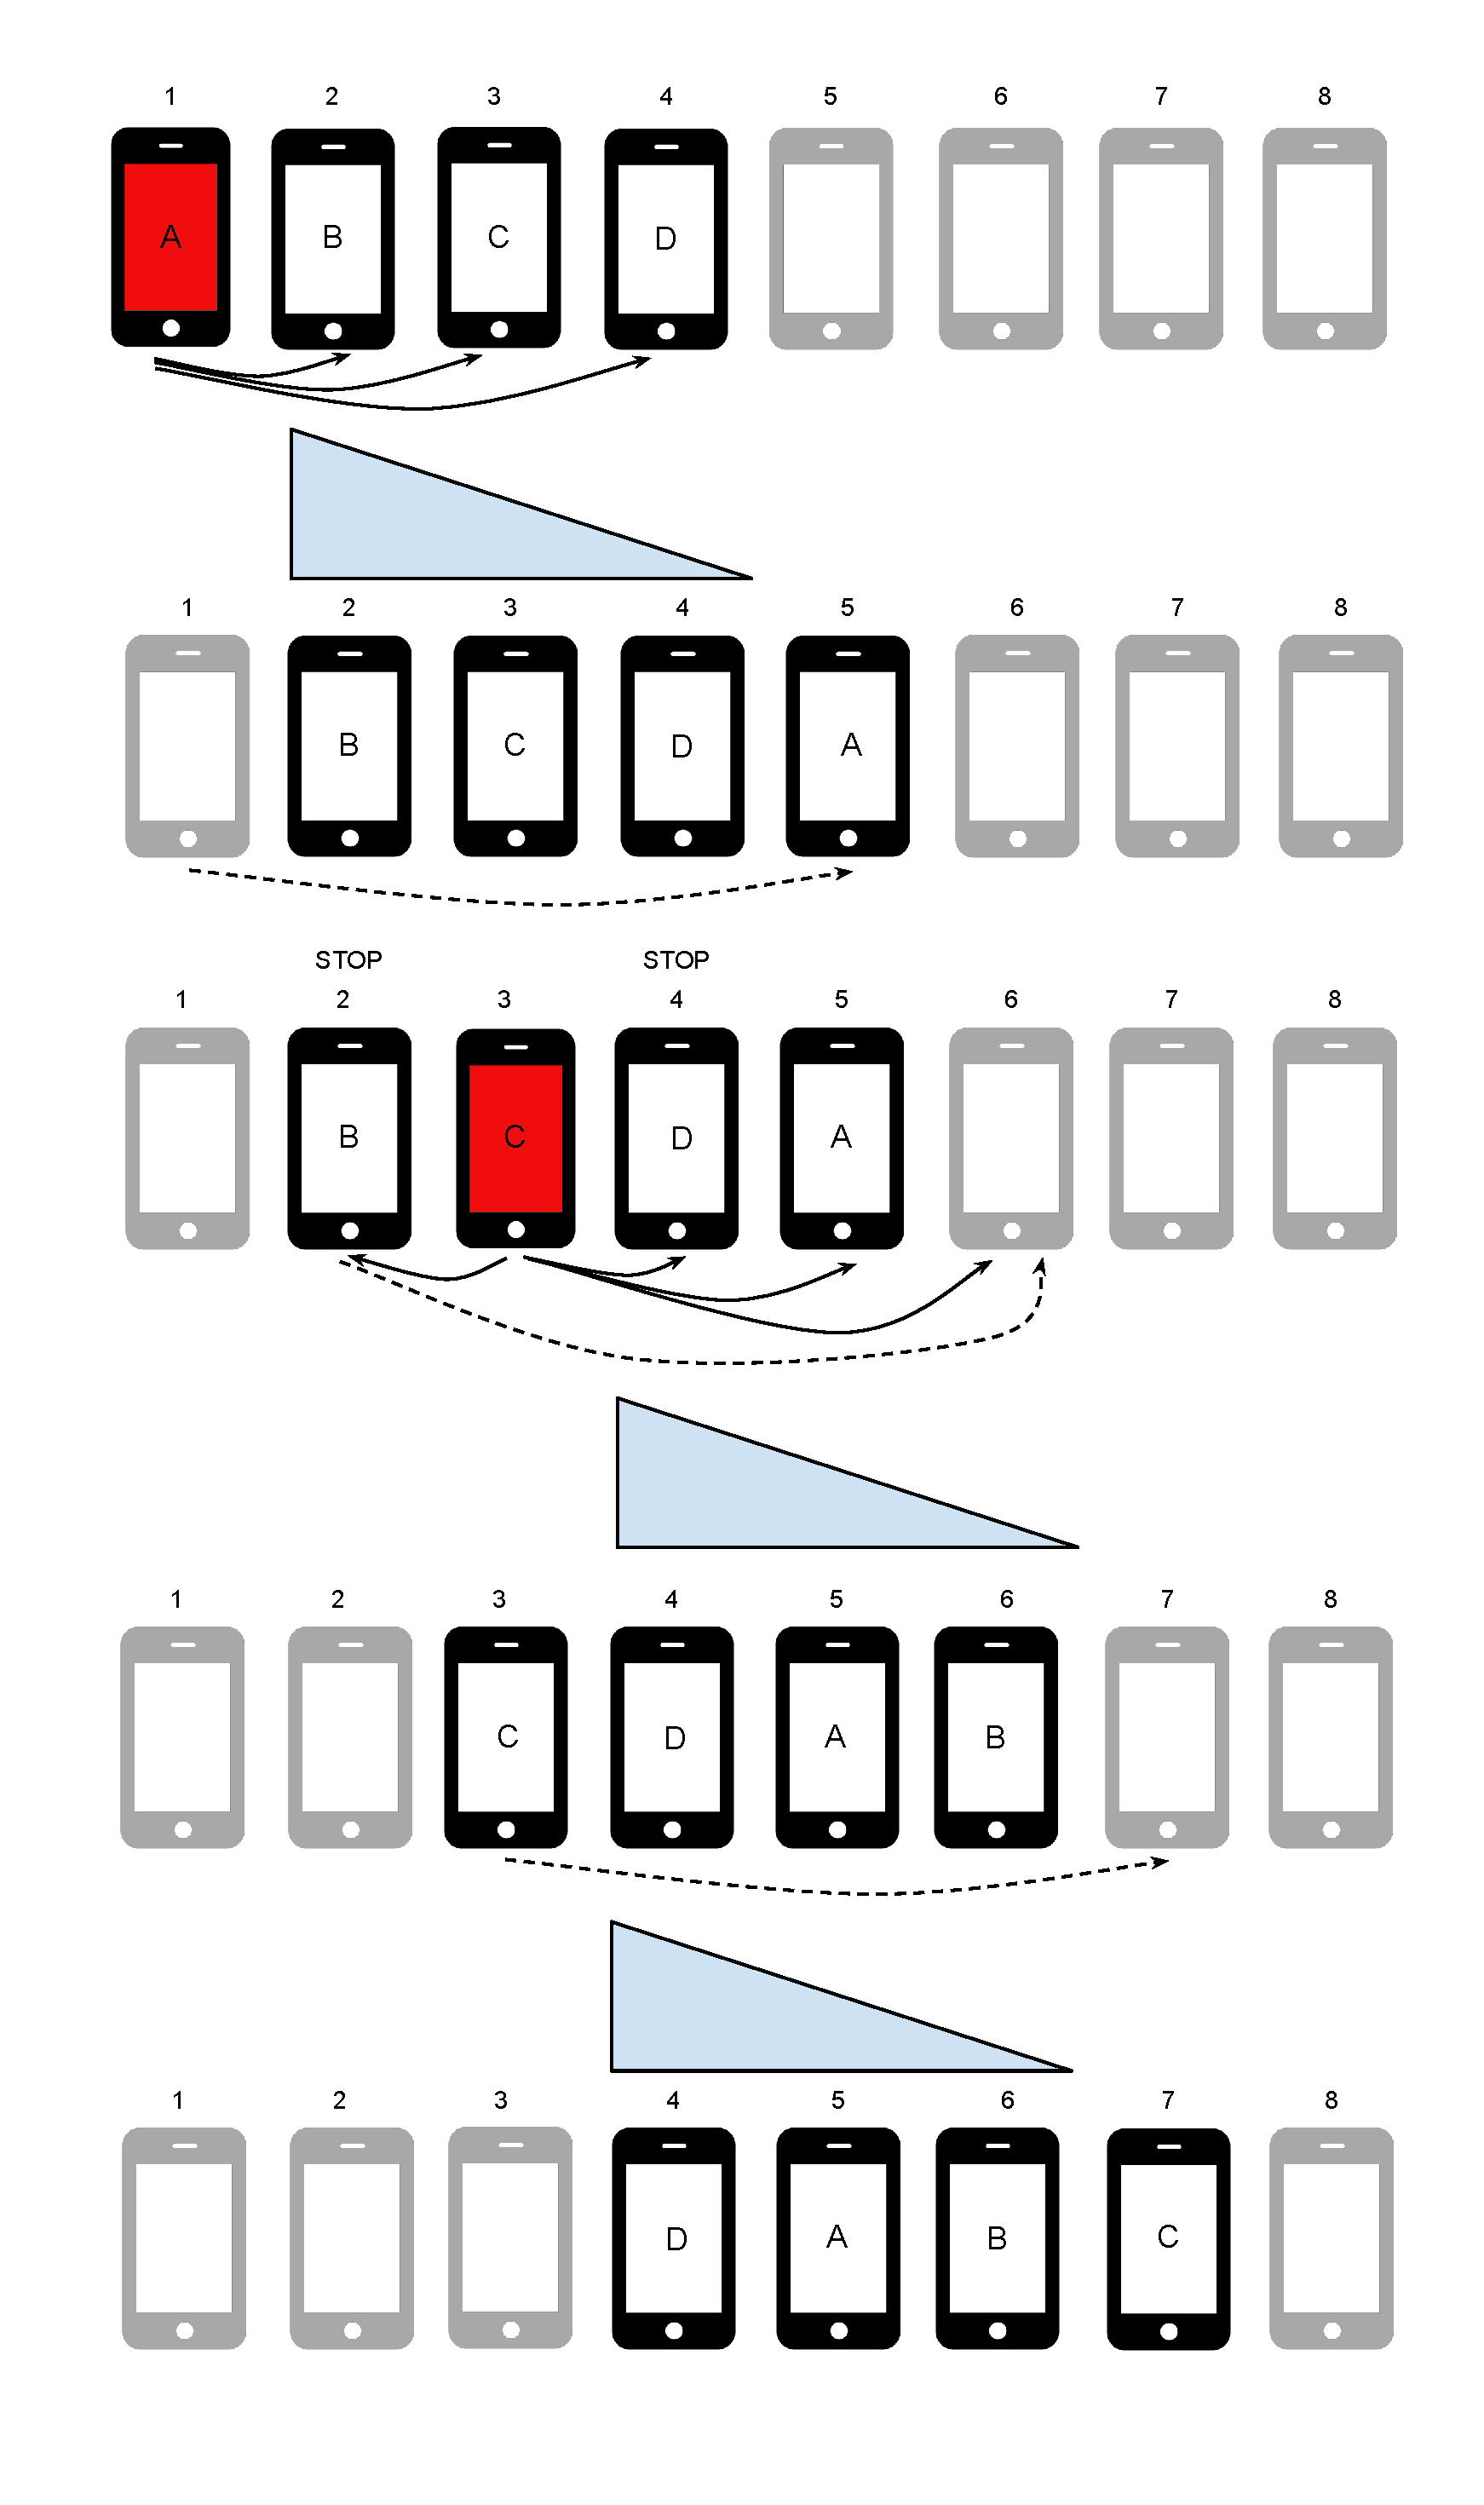
\includegraphics[trim = 10mm 15mm 10mm 10mm ,width=3.5in]{imgs/Positions_1.pdf}
\caption{Devieces position changes}
\label{fig:positions}
\end{figure}
